\chapter{Translation and Static Analysis}
	What is translation (mathematically speaking)? Let $\Sigma$ and $\Delta$ be two alphabets (\emph{source} and \emph{target} respectively); a translation is a correspondence between source and target strings, that is formalized by binary realtion between the source and target universal languages (that is $\Sigma^\ast$ and $\Delta^\ast$). Formally, a translation is a subset of $\Sigma^\ast \times \Delta^\ast$. So, it can be also seen as a function, and inherits all the function's peculiar properties (like surjectivity, injectivity and all the terminology that concerns dominion, image and inverses).
	
	\section{Purely Syntactic Translation}
		\subsection{Translation Grammars}
			When the source language is generated by a grammar, one of the most natural translation is to map each subtree to a target subtree. This is done by building a \emph{translation grammar} that have the same number of rules of the source language grammar and differs only in the terminal symbols in the right part of the rules. The nonterminals symbols are \emph{the same and in the same order}.\\
			A typical example of translation grammars come from bynary functions notation, when translatin the classic infix notation ($A \times B$) into a pre/postfix polish notation, like $\times A B$ that's way more concise and understandable, being less prone to error caused by operator's precedence.\\
			We have so a grammar for the infix notation expression, and one that describes the target language, a prefix polish notation:
			\begin{equation}
				\begin{cases}
					E \rightarrow E + E \\
					E \rightarrow E * E \\
					E \rightarrow ( E ) \\
					E \rightarrow i
				\end{cases} 
				\begin{cases}
					E \rightarrow \text{add } E \text{ } E \\
					E \rightarrow \text{mult } E \text{ } E \\
					E \rightarrow E  \\
					E \rightarrow i
				\end{cases}
			\end{equation}
			So we build our translation grammar this way:
			\begin{equation}
				\begin{cases}
					E \rightarrow \frac{\epsilon}{add} E \frac{+}{\epsilon} E \\
					E \rightarrow \frac{\epsilon}{mult} E \frac{*}{\epsilon} E \\
					E \rightarrow \frac{(}{\epsilon} E \frac{)}{\epsilon} \\
					E \rightarrow \frac{i}{i} \\
				\end{cases}
			\end{equation}
			
			\subsubsection{Ambiguity}
				If the source grammar is ambiguous then the translation scheme is ambiguous: if a sentence can be generated bby more than one syntax trees, obviously the translator should take care of this multi-valued rules. Ambiguity in the translation grammar can also derive by duplicated rules, that can be mapped to different values: in this case, both the source and target grammar are unambiguous, but multiple translation rules correspond tothe same source rule, rendering the translation grammar multi-valued $\Rightarrow$ ambiguous.\\
				Summing up these two concepts, a translation grammar $ G_\theta = \{ G_1 , G_2\}$ is unambiguous (single-valued) if 
				\begin{enumerate}
					\item $G_1$ is unambiguous;
					\item No two rules of target grammar $G_2$ map on the same $G_1$ rule.
				\end{enumerate}
		
		\subsection{Pushdown Transducer}
			We have defined a translation between grammars, now we have to define a machine that performs it. Such machine is a \emph{pushdown transducer}, so a pushdown automaton with output capabilities. It has the same definition of a PDA, enriched with the output (target) alphabet, and with a different transiction function: in fact, this should now take into account also the output of the machine, not only the state transitions.\\
			\emph{A translation relation is defined by a translation grammar iff it is computed by a nondeterministic pushdown transducer}. This property ensure the equivalence of the two methods, and also grants the possibility of defining a machine starting from the grammar as in traditional parsing. 
			
			\subsubsection{Single state nondeterministic transducer}
				Theoretically speaking, the simplest extension from a parser to a transducer is built directly associating to the grammar rules some move, this time adding the write operation. We obtain a nondeterministic single state transducer, with not the minimal practical value.
			
			\subsubsection{ELL grammars translation}
				ELL parsers can be implemented by recursive function calls (classic top down approach), as explained in (21.4.3). Extending the recursive calls parsers with write functions just after the submodule call is enough to render the parser a transducer. Simple as that. Remember that ELL parsers rely on a stronger assumption then ELR, so they're less complex and easier to extend; they're also applicable to a reduced number of cases.
			
			\subsubsection{ELR grammars translation}
				ELR parsers are not easily extended as their ELL brothers. In fact, just adding the output action after a shift operation could lead to contradictory writes, becaouse of the inherent nondeterminism of the bottom up approach to parsing. Instead, the reduce operation grants the recognition of a single grammar rule, and (due to the total mapping of the source to the target rules) one target rule can be identified and selected for output.\\
				This is easier said than done: a reduction could take place before another that may need to write a characte \emph{before} the current one; to avoid this kind of phenomena, the translation grammar must be in \textbf{postfix normal form}: a translation grammar is in postfix normal form when all its rules are of the kind
				\begin{equation}
					A \rightarrow \Sigma^\ast \delta^\ast
				\end{equation} 
				so they produce the output strings \emph{only} at the end of the rules as a suffix of the production, and not in the middle of it.\\
				To convert a grammar in the postfix normal for it's enough to replace all the terminals in the translation that violates the postfix form with new nonterminals that simply produces the substitued character (this change should be reflected in the target grammar also). A translation grammar in the postfix normal form ensures that, when implemented via an automaton, the output operations take place only at reduction time. This trnsformation makes sure that the construction of a pilot automaton for a \emph{transducer} is identical to the one for a \emph{parser} with just the write operation added to the m-states that have a final state in them.\\
				In some particular cases (that are indeed very rare, according to the literature) normalizing a grammar can introduce shift reduce conflicts due to the introduction of initial - final states in the automaton.
			
			\subsubsection{Regular Translation}
				\paragraph{Regular Languages Translation}
					As regular expression are a proper subset of CF grammars, they have a special family of transducers. Consider this translation grammar:
					\begin{equation}
						G_\tau = 
						\begin{cases}
							A_0 \rightarrow \frac{a}{c}A_1 \,\vert\, \frac{a}{c} \,\vert\, \frac{a}{b}A_3 \,\vert\, \epsilon \\
							A_1 \rightarrow \frac{a}{c}A_2 \,\vert\, \epsilon \\
							A_2 \rightarrow \frac{a}{c}A_1 \\
							A_3 \rightarrow \frac{a}{b}A_4 \\
							A_4 \rightarrow \frac{a}{b}A_3 \,\vert\, \epsilon 
						\end{cases}
					\end{equation}
					\textbf{Things to be noted}:
					\begin{enumerate}
						\item the grammar translates string of "a" in strings of "b" when the number of "a" is even
						\item the grammar translates string of "a" in strings of "c" when the number of "a" is odd
						\item to "count" the number of letters, the grammar constructs two loops ($A_0 \rightarrow A_1 \rightarrow A_2 \rightarrow A_1$ and $A_0 \rightarrow A_3 \rightarrow A_4 \rightarrow A_3$) to either create an odd number of letters or an even one. This can be noted observing which rules contains the empty string in the loop
						\item the grammar is right linear (so? it's equivalent to a regular expression)
						\item the grammar is in prefix normal form (does this have some relevance now? no)
					\end{enumerate}
					As well as a right linear grammar can easily be converted in a regular expression, we can derive a \emph{regular transducer} that translates the language of this translation grammar. It's pretty straightforward:
					\begin{equation}
						e_\tau = \left(\frac{a^2}{b^2} \right)^\ast \,\cup\, \frac{a}{c} \left(\frac{a^2}{c^2} \right)^\ast
					\end{equation}
					
				\paragraph{Two Input Automaton}
					Starting from the defined "regular translator" in the previous paragraph, we can see that the combination of terminals of the source and target expressions can be seen as a terminal alphabet itself (it will be a terminal alphabet built on the cartesian product of two alphabets, but the idea is there). So, with the regular expression $\leftrightarrow$ FSA equivalence in mind, we can define a FSA that recognize (validates) the translations of the source expressions. This machine will ha ve \emph{two} input tapes, one for the source and one for the target terminals, and will recognize the input when it's a valis translation. The only thing that's odd about 2I-FSA is the way empty strings are managed: if the transiction function accepts a empty string as input character \emph{on one of the two tapes}, the machine could still be blocked by the reading on the other one.\\
					As an example we produce the 2I-FSA that recognizes the translation of the above regular translation.
					\begin{figure}[H]
						\centering
						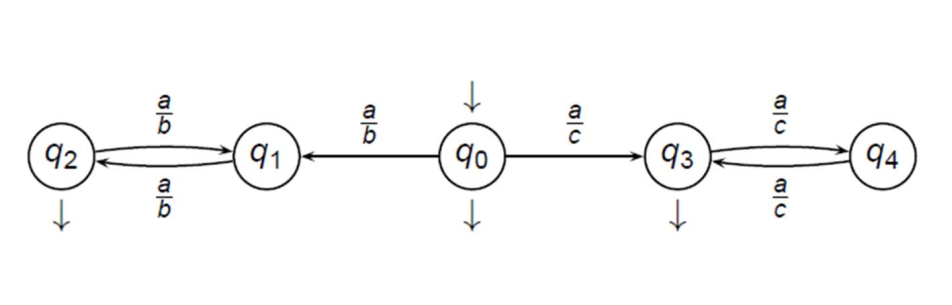
\includegraphics[width = \textwidth]{./images/2IFSA.png}
						\caption{To be noted: this automaton is deterministic, because the two moves exiting from $q_0$ have different labels}
					\end{figure}
					
				\paragraph{Finite Transducer}
					We want an automaton that formalizes the translation (REMINDER: A 2I-FSA DOES NOT TRANSLATE, BUT VALIDATES A TRANSLATION) so that starting from a string on an input tape prints the translated string on an output one. The schema is very simple:
					\begin{figure}[H]
						\centering
						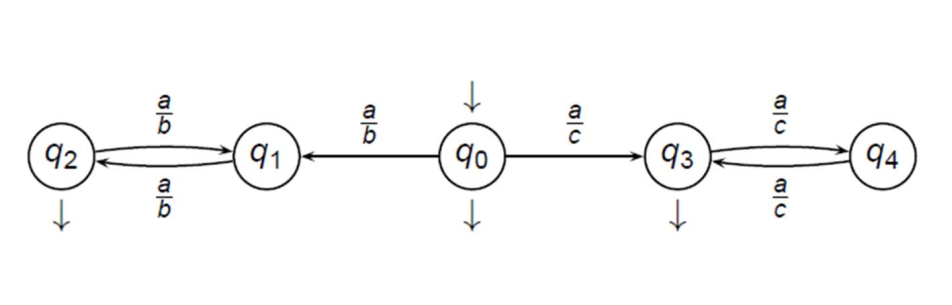
\includegraphics[width = \textwidth]{./images/2IFSA.png}
					\end{figure}
					Is it familiar? It's the \emph{same} formalization as the 2I-FSA that validates the translation, but this time the labels have a \textbf{totally different meaning}: the bottom character represents the one printed on the output tape. So, this time the automaton is nondeterministic, because of the two arcs exiting from $q_0$ have the same input character; only one of the two will make the automaton finish in an acceptance state; this also means that \emph{no output can be produced until a final state is reached}.
					
				\paragraph{Sequential Transducer}
					Ok, now we want a machine that translates input \emph{real time}, so while scanning the input tape (to overcome the limitation of finite transducers that must reach a final state to print). The sequential transducer model differs from the aforementioned ones in the theoretical representation (it makes use of three functions: a transition one, an output one, and a \emph{final} one) but not in the graphical rep. The core idea is very similar to the finite transducer but the output characters are \emph{actually} printed as output. This model needs an additional function that computes the "string terminator": the so called final function, in fact, just appends to the translated string a marker that signals the end of the translation, and the final state reached by the computation.\\
					This may seem overly complicated, let's use an example to clarify: a sequential transducer that eliminates all the leading zeroes from a string. The input string are built on a alphabet composed of three characters, \{ $0, 1, \sqcup$ \} where $\sqcup$ represents the separator between values. If a string is composed solely by zeroes, a single zero is outputted.
					I'll skip the definition of the regular translation expression for this automaton, to present directly the machine:
					\begin{figure}[H]
						\centering
						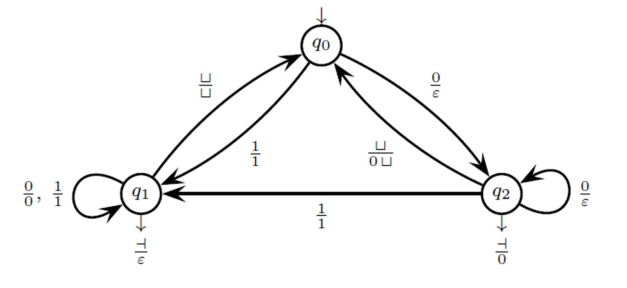
\includegraphics[width = \textwidth]{./images/SeqTrans.png}
					\end{figure}
					The above machine can be explained section by section:
					\begin{enumerate}
						\item state $q_2$ carries out the meaningless zeroes. She outputs nothing, never, exception made for when the terminator is read, when a single zero is written. 
						\item state $q_1$ takes care of the meaningful part of the string. It's reachable through a scan of the character "1", that signals the start of the meaningful part of the string; its only task is to traduce the string as is.
						\item $q_0$ interpret blank spaces. 
					\end{enumerate}
					
	\section{Syntax Directed Translation}
	
		The compilation process cannot be performed only through syntactic methods. A \emph{meaning} must be assigned to sentences, and (while this can be accomplished in a formal way) the only "structured reading and translation" of a sentence is not enough to do so. Syntax directed translators starts from the syntax trees of a grammar and enrich them with semantic attributes. 
		
		\subsection{Attribute Grammars}
			Attribute grammars have the same computing expressiveness of Turing machines (they are very powerful). They are the third step of computations during a compilation procedure: they are preceded only by lexical and syntactic analysis. The purpose of attribute grammars is to help design the \emph{decorated syntax tree} that enriches the normal s.t. with a semantic value.\\
			Let's run an example:
			
			\paragraph{Meaningful example}
				We'll build an attribute grammar for the language $L = \{0, 1\} \,\bullet\, \{0, 1\}$ that represents decimal numbers in a fixed point fashion. The grammar that generates it is
				\begin{equation}
					G_L = 
					\begin{cases}
						N \rightarrow D \bullet D \\
						D \rightarrow D \, B \, \vert \, B \\
						B \rightarrow 0 \, \vert \, 1
					\end{cases}
				\end{equation}
				Where N is the axiom, D is the string, B is the single bit. The goal of our attribute grammar is to compute the decimal value of each part of the number, assigning the real weight to the single bits. To do so, we need to keep track of two fundamentals attributes:
				\begin{enumerate}
					\item The value of the numeric parts of the string: the N, D and B nonterminals have all this attribute, because they are all \emph{semantically} numbers;
					\item Their position in the string; an easier way to compute so is to keep track of the string lenght. Only nonterminal D needs this attribute. N does not need it because it's just a concatenation of two values. 
				\end{enumerate}
				So, now we have a grammar and a set of attributes with a semantic value that must be linked to certain nonterminals. To do so, we can define functions (associated to every production) that computes the value of the nonterminal of the reduction. In this case:
				\begin{equation}
					G_{L_ext} = 
					\begin{cases}
						N \rightarrow D \bullet D \text{ sum of the right with the left part: } v_0 = v_1\,+\,v_2\times 2^{-l_2} \\
						D \rightarrow D \, B \, \vert \, B \text{ also consider the length increase: } 
							\begin{cases}
								\begin{cases}
									v_0 = 2 \,\times\, v_1\,+\,v_2 \\
									l_0 = l_1 + 1
								\end{cases}\\
								\begin{cases}
									v_0 = v_1 \\
									l_0 = 1
								\end{cases}
							\end{cases}\\
						B \rightarrow 0 \, \vert \, 1 \text{ just assign the final value to the nonterminal: } 
							\begin{cases}
								v_0 = 0\\
								v_0 = 1
							\end{cases}
					\end{cases}
				\end{equation}
				A detailed explanation of what $l_0, l_1, v_0, v_1 \text{ and } v_2$ are is needed: the letter is the attribute we're referencing ($l = \text{ lenght and } v = \text{ numeric value}$) and the pedix symbolizes the \emph{cardinal position of the nonterminal we are considering}: this means that all the attributes that have the zero pedix will be the results of the computation, because they are the attributes of the left part of the grammar rule. Vice versa, $v_2$ represents the numeric value of the \emph{third} nonterminal in the rule.\\
				The computation evolves around the tree in this way:
				\begin{figure}[H]
					\centering
					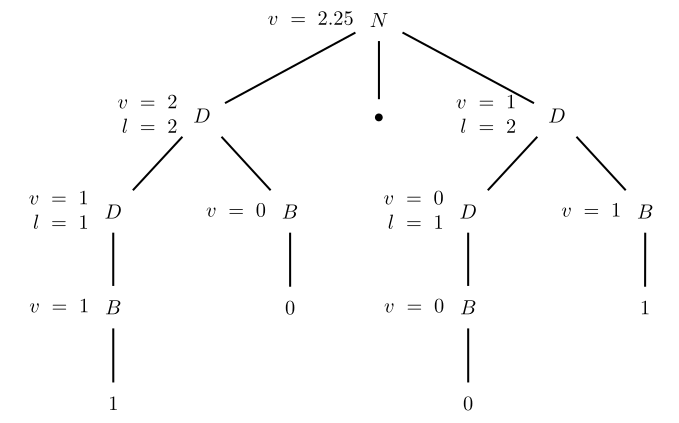
\includegraphics[width = \textwidth]{./images/decoratedTree.png}
				\end{figure}
				
			\subsubsection{Left and Right Attributes}
				The definition of left and right attributes is as tricky as fundamental for the comprehension of attribute grammars. Let's try to figure it out:
				\paragraph{Left attributes}
					We want to generate a value from a production, what did we do in the previous example? We computed the value for the right part recursively till a fixed point (the production that has associated a function that produces a costant, such as $l_0 \,=\, 0$). In this case, $l_0$ is a left attribute, because it's associated with a left part of the rule. Left attributes are also called "synthetized" because they usually represents the result of the computation.
				\paragraph{Right attributes}
					We say that an attribute is "right" or "inherited" if it's associated to a right part of a rule, so the functions that calculate it has as output not a value that goes in the left part of the rule, but stays in the right part.  
				\\\\Still nebolous definitions, and no practical value. Let's make an example, \emph{read it carefully}:\\
				we have as input a string of words, separated by blank spaces (we will represent them with $\dashv$). We want to arrange the text into rows of fixed length $W$ and compute for each word the column of its last character. We assume no words have length that's greater than $W$. 
				\begin{equation}
					G = 
					\begin{cases}
						S \rightarrow T \\
						T \rightarrow T \dashv T \\
						T \rightarrow V \\
						V \rightarrow cV \,\vert\, c
					\end{cases}
				\end{equation}
				The "c" terminal respresents any character. Which attributes are needed?
				\begin{itemize}
					\item \emph{last} stores the column of the last letter
					\item \emph{length} stores the length of the word
					\item \emph{prec} is the column of the last character of the previous word
				\end{itemize}
				These three attributes are all we need to describe the set of words, element by element. The idea is to compute the last character of each word as: $last = prec + 1 + lenght$. It's pretty straightforward spotting the only right attribute: \emph{prec}. In fact, it's extracted from the left part of the rule. Let's define all the functions associated to the rules.\\\\
				\begin{center}
					\begin{tabular}{| m{3cm} || m{3cm} | m{3cm} | }
						Rule & Left attributes & Right attributes \\
						\hline
						$S \rightarrow T$ & & $prec_1 = -1$\\
						\hline
						$T \rightarrow T \dashv T$ & $last_0 = last_2$ & $prec_1 = prec_0\,\,\,prec_2 = last_1$ \\
						\hline
						$T \rightarrow V $ & $last_0 = (prec_0 + lenght_1 + 1 > W) ? lenght_1 : (prec_0 + lenght_1 + 1)$ &\\
						\hline
						$V \rightarrow cV$ & $lenght_0 = 1 + lenght_1$ & \\
						\hline
						$V \rightarrow c$ & $lenght_0 = 1$ &  
					\end{tabular}
				\end{center}
				Let's describe what's each function do:
				\begin{itemize}
					\item Left attributes:
					\begin{itemize}
						\item $last_0 = last_2$ stands for "the last element of two words is the last element of the last word".
						\item $last_0 = (prec_0 + lenght_1 + 1 > W) \,?\, lenght_1 \,:\, (prec_0 + lenght_1 + 1)$ this function (expressed as a inline if instruction) verifies if we've reached the end of the line, composed of $W$ coloumns. If we are (the condition is true) we've reached the first word of the next line, so the lasta character of this word will be on the last coloumn. Otherwise, it will be taken into account also the lenght of the preceding word.
						\item  $lenght_0 = 1 + lenght_1$ and $lenght_0 = 1$ are classical recursive calls to form the words lenght.
					\end{itemize}
					\item Right attributes:
						\begin{itemize}
							\item $prec_1 = -1$ initializes the first word's predecessor.
							\item $prec_1 = prec_0$ and $prec_2 = last_1$ sets the value of the predecessor for each word. Note how the information, in this case, flows downward to the leaves: to be set are the values of attributes that only later in the execution will be utilized. In this case: we're setting the predecessor of each word: predecessor of the first = last one's predecessor and second one's predecessor = last character of the first.
						\end{itemize}
				\end{itemize}
				The final decorated tree is:
				\begin{figure}[H]
					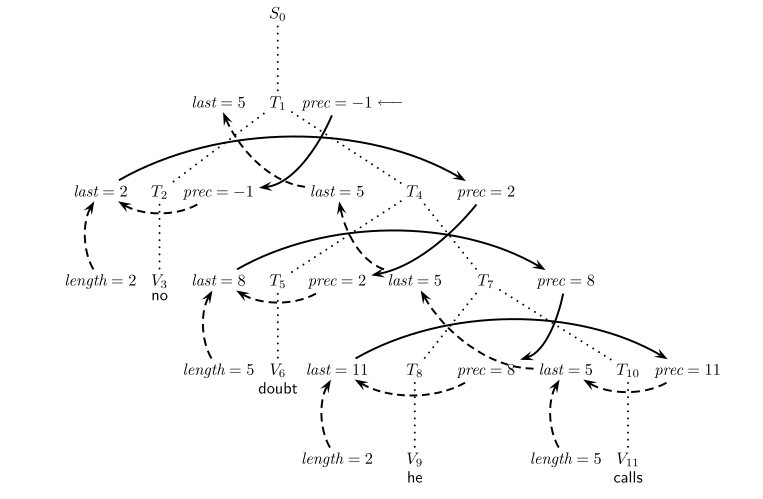
\includegraphics[width = \textwidth]{./images/decTree.png}
				\end{figure}
				Let's formalize all this reasoning:
			
			\subsubsection{Formal Definition of an Attribute Grammar}
				An attribute grammar is composed of:
				\begin{enumerate}
					\item A context-free grammar $G = \langle V, \epsilon, P, S \rangle$ with her set of terminals, nonterminals and the axiom. It is convenient to NOT have the axiom in the right part of the rules
					\item A set of semantic attributes, associated with terminals and nonterminals. This set is separated in left attributes and right attributes: \emph{the two sets are disjoint. No right attribute can be left attribute in another production and vice versa}. The set of attributes of nonterminal D is also referred to as $attr(D)$
					\item A set of semantic functions, each associated with a grammar rule. The grammar rule associated with each function is called the support of that function. In general, several functions can have the same support, and the set of functions supported by production p is $fun(p)$. Semantic functions are formally defined as:
						\begin{equation}
							\begin{cases}
								\text{the support: } p = D_0 \rightarrow D_1 D_2 ... D_r\\
								\text{the function: } \sigma_k = f(attr(\{D_0, D_1, ..., D_r\}) \backslash \{\sigma_k\})\\
								r \geq 0\\
								0 \leq k \leq r
							\end{cases}
						\end{equation}
					\item All the semantic functions must respect:
						\begin{enumerate}
							\item For each left attribute of a left nonterminal of a production there is \emph{exactly one} function that defines it
							\item For each production, no functions defines \emph{right attributes for the left side nonterminals}
							\item For each production, no functions defines \emph{left attribute for the right side nonterminals}
							\item For each right attribute of a right nonterminal of a production there is \emph{exactly one} function that defines it
						\end{enumerate}
						These four rules better regulates the "attributes placements and initialization": in fact, they states that all the left-hand side nonterminals can have only left attributes and also that such attributes must be uniquely defined; also they states that for all right-hand side nonterminals only left attributes are possibly defined and \emph{also} they are uniquely defined. The other attributes are called \emph{external attributes}, because they're not comupted in the function.\\
				\end{enumerate}
				
				\paragraph{Dependence Graph}
					The graph showed in 23.1.1 is a complete dependence graph obtained by "summing" all the graphs of its subtrees. The single dependence graph can be referred to semantic functions, or to productions (so \emph{to all} the semantic functions that have that rule as support). The decorated syntax tree, ultimately, is the complete dependence graph of all the productions.\\
					How to build a decorated tree, even though it's far from Christmas: just link the arguments of the function to the attribute that function initializes. So, if the function is $attr_0 = f(\{attr_1, attr_2\})$ in the decorated graph we will have something like $attr_1 \rightarrow attr_0 \text{ and } attr_2 \rightarrow attr_0$.
			
			\subsubsection{Grammar Validation}
				Given an attribute grammar defined as before, if the dependence graph of the tree is acyclic, there's a set of attribute values consistent with the dependences. A grammar is loop free id \emph{every dep graph of every tree} is acyclic. How to test if a grammar is acyclic? Given the infite number of syntax trees, computing all of them to check for cycles is not viable. Instead, it's enough to ensure certain properties, that are sufficient to guarantee the desired condition of acyclicity.
				
				\paragraph{One Sweep Grammar}
					"One sweep" is a property that ensures that a grammar can be evaluated with a depth first visit. What does this mean? It means that \emph{it's possible to perform attribute evaluation during a depth first visit}. Why should this be checked? Because the depth first visit operates this way:
					\begin{enumerate}
						\item before entering a subtree compute all right attributes of the root of that subtree
						\item when "emerging" from a visit of a subtree, compute all the left attributes of the root of that subtree
					\end{enumerate} 
					Both these two operations can get stuck in the evaluation of certain attributes, because of the possible functional dependences among attributes. A one sweep grammar is ensured to be free of such problems.\\
					So how to check for "onesweepness"? We shall recall the definition of the $dep$ set, and introduce the \emph{sibling graph}:
					\begin{enumerate}
						\item The nodes are the right symbols of the productions $\{D_1\,...\,D_r\}$.
						\item Arcs $D_i \,\rightarrow\, D_j$ are drawn between nodes that have an attribute dependency like $\sigma_{D_i} \,\rightarrow\, \theta_{D_j}$. The nodes in the siblings graph \textbf{are not} the ones of the dependence graph of the production. 
					\end{enumerate}
					Let's generate a sibling graph for a dummy rule, $D\rightarrow A\,B\,C$ that has the dependency graph as below:
					\begin{figure}[H]
						\centering
						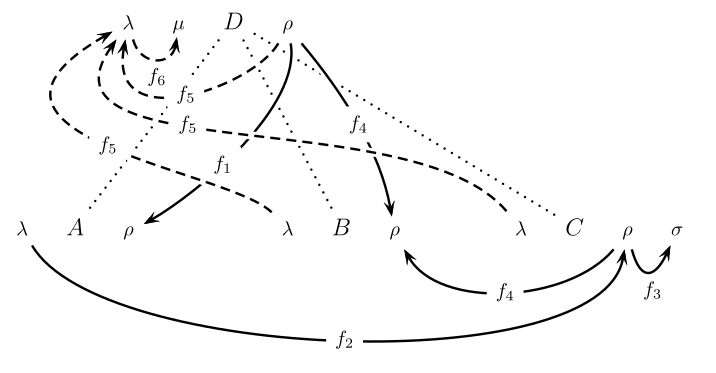
\includegraphics[width = \textwidth]{./images/dummyRule.png}
					\end{figure}
					The resulting sibling graph is:
					\begin{figure}[H]
						\centering
						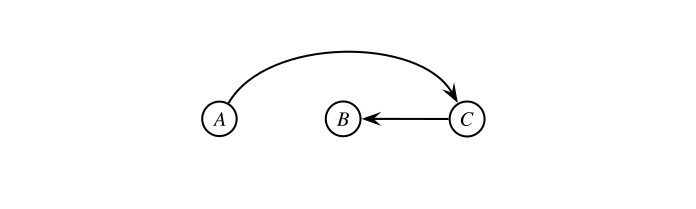
\includegraphics[width = \textwidth]{./images/sibling.png}
					\end{figure}
					For a grammar to have the one sweep property it must hold, for all the productions:
					\begin{enumerate}
						\item $dep_p$ contains no circuits;
						\item $dep_p$ contains no path that goes from a left attribute to a right attribute of the same node;
						\item $dep_p$ contains no arc from the left attribute of a father to a right attribute of a children;
						\item $sibl_p$ contains no circuits. 
					\end{enumerate}
			
			\subsubsection{Validation of a Grammar through a One Sweep Evaluator}
				The algorithm we described before to visit a tree depth first can be formalized to generate a one sweep evaluator, a machine that carries out all the computation of an attribute grammar. REMEMBER: the evaluator built this way \emph{relies} on the assumption that the grammar is one sweep.\\
				A semantic procedure is written for each \emph{nonterminal}: this procedure has as arguments the subtree generated by that nonterminal and his right attributes. The procedure must, for every support rule $p: D_0 \,\rightarrow\, D_1\,...\,D_n$ with $n \geq 0$
				\begin{enumerate}
					\item Choose the TOS (Topological Order for Siblings) for $\{D_1\,...\,D_n\}$ wrt the sibling graph for that nonterminal
					\item Choose the TOR (Topological Order for Right attributes) for all the right attributes of all symbols $\{D_1\,...\,D_n\}$ wrt the dependence graph of that symbol
					\item Choose the TOL (you guess. Hint: opposite of right...)
				\end{enumerate}
				These three \st{demigods} orders prescribe \emph{how to arrange the instructions} in the procedure body. To explain that, we'll make as example the procedure that is generated by the rule in the previous example, $D \,\rightarrow\, A\,B\,C$, with the dep graph as shown before. This grammar is easily proven one sweep (the sibling graph has no cycles and no cycles or cross dependecies are seen in the dep graph).\\
				The procedure starts of choosing a TOS: due to the sibling graph's arcs, the order choosen is $\{A,\,C,\,B\}$.\\
				Then she chosses the TOR, taking into consideration the dependencies shown in $dep$: $\rho\,\rightarrow\,\sigma$ is the one.\\
				Last but not least TOL: again, watching the dependencies, we have $\lambda\,\rightarrow\,\mu$.\\
				Once these three orders are identified, the procedure can be written: I'll try to give an abstract explanation of \emph{how} the three orders are used (because I hate pseudocode) then I'll add a pseudocode example.\\
				Subtrees are computed in TOS order, and for each subtree the "computational pattern" is
				\begin{enumerate}
					\item compute right attributes in TOR order using the functions highlighted in $dep$
					\item call the subprocedure of that symbol passing as argument also the attribute to popolate
					\item compute left attributes with the assigned functions in TOL order
				\end{enumerate}
				
				So in this case, the procedure becomes:\\
				def D ( in: root, $\rho_D$, out: $\lambda_D$, $\mu_D$):\\
			    $\rho_A = f_1(\rho_D)$\\
			    $A(root_A, \rho_A; \lambda_A)$\\\\
				$\rho_C = f_2(\rho_A)$\\
				$\sigma_C = f_3(\rho_C)$\\
				$C(root_C, \rho_C, \sigma_C; \lambda_C)$\\\\
				$\rho_B = f_4(\rho_C, \rho_D)$\\
				$B(root_B, \rho_B; \lambda_B)$\\\\
				$\lambda_D = f_5(\lambda_B, \lambda_C, \rho_D)$\\
				$\mu_D = f_6(\lambda_D)$\\
	
	\subsection{Combined Syntax and Semantic Analysis}
		In some cases syntax analysis and attribute evaluation (semantic analysis) can be performed at the same time. For each class of languages we've seen, a different approach can be developed.
		
		\subsubsection{Regular Laguages - Lexical Analysis with Attribute Evaluation}
			If the language is regular, then the \emph{scanner} or \emph{lexxer} 's task is to identify and isolate \emph{lexemes}, the minimal tokens of a language that can be given a semantic weight. The scanner can also give attributes to these tokens, and compute them.
		
		\subsubsection{LL Languages - Attribute Recursive Descent Translator}
			If the syntax is suitable for top down parsing (is LL) and the grammar is one-sweep, it's necessary to add just another hypothesys to make sure that the parsing and the semantic analysis can procede step by step together. The condition to be satisfied is the L condition, that states:\\
			a grammar satisfies the L(eft to right) condition if
			\begin{itemize}
				\item It's one-sweep
				\item The sibling graph (of every support) contains \textbf{no arc} so that $D_i \,\rightarrow\, D_j$ with $j > i \geq 1$ (so no \emph{backward dependency})
			\end{itemize}
			If the syntax is LL and the L condition is satisfied (what is wrong with the letter L I would like to know) then a \emph{attribute recursive descent translator} can be built \footnote{I know, it sounds like a General Zod weapon, doesn't it?}.\\

    \section{Static Analysis}
            \subsection{Compilation of a Program}
                Compilers are composed of two part: a front end compiler (that translates the actual source code into a "lower level code". This is made possible by a scanner + parser pipeline) and a back end compiler (that takes the lower level code and generates the executable). After the front end compiler has generated the intermediate representation of the program, this goes through three additional phases:
                \begin{enumerate}
                    \item \textbf{Verification} correctness check
                    \item \textbf{Optimization} target specific improvements to enhance performance
                    \item \textbf{Scheduling} modification of the produced code to fully use the pipelines/parallel capabilities of the machine
                \end{enumerate}
                
                \subsubsection{Control Flow Graph}
                    To analyze the program in these three further phases, a schematic representation of the program itself is needed. This representation is usually a control flow graph, that stands for an automaton. Needless to say, this automaton is the same \emph{formal structure} of the ones used to interpret the source code, but has a \emph{totally diffferent meaning}: this automaton in fact describes the program itself and the use it makes of the variables.
                    
                    \paragraph{How to Build a CFG}
                        CFGs are simple def-use graphs. They do \emph{not} represents the logic unfolding of the program, but just the usage of the memory. The following abstractions are utilized:
                        \begin{itemize}
                            \item All the conditional statements are not represented
                            \item "Instruction B follows instruction A" is drawed out as the classic arc
                            \item All operations are reduced to two sets: \emph{def} and \emph{use}. These two sets represents the group of variable to which a value is assigned and the group of variables which value is read
                        \end{itemize}
                        So far, we've defined an automaton with some sets. But which strings does this automaton recognizes? A string recognized by an automaton described by means of a CFG is a possible \emph{execution trace} of the program, or the execution path that traverse a valid sequence of instructions. In these pages, we will consider onyl \emph{intraprocedural} static analysis, that is performed \emph{in isolation} on every procedure.
                    
                    \paragraph{Conservative Approximation}
                        The choice to ignore the unreachable path enables the analyzer to reach unreachable segments of code. This could lead to pessimistic outcomes (like a program is deemed invalid or with errors, but these errors are all located in an unreachable segment). This condition is called conservative approximation because "pessimistic conclusions" are far preferrable rather than "optimistic conclusions": the latter can lead to assign a smaller-than-needed amount of resources, while the former never misses an error.
                
                \subsubsection{Liveness Intervals Analysis}
                    Variable liveness analysis is used to discover definition errors or clashes or unreferenced accesses. A variable \emph{a} is said to be "live" on the \emph{exit} of a node \emph{p} if there exists a path between \emph{p} and another node \emph{q} so that \emph{a} does not appear in \emph{any} def sets of the traversed nodes, but it appears in the use set of \emph{q}.\\
                    This definition is usually referred to as "live-out", because it takes in consideration the exiting arcs from a node. A specular formulation ("live-in") can be given. Example of usage: if a variable is defined in a certain node, but it's not live-out of that node, the assignement can be deleted without altering the program behaviour.
                    
                    \paragraph{Computing Liveness Intervals - Data Flow Equations}
                        The scary name of "data flow equations" is given to a rather simple approach to the problem of calculating all the $live_in$ and $live_out$ sets for each node of the control flow graph. The procedure is inherently recursive and starts from the final nodes. It unfolds this way:
                        \begin{equation}
                            \forall p \in CFG \,\vert\, p \in Finals \Rightarrow live_{out}(p) = \emptyset
                        \end{equation}
                        So (quite logically) if a node is final his live out variable set is empty. Next equation (that represents the "recursive call") makes use of the $succ$ set, representing all the \emph{immediately reachable nodes} from a given one.
                        \begin{equation}
                            \forall p \in CFG \,\vert\, live_{out}(p) = \bigcup\limits_{\forall q \in succ(p)} live_{in}(q) 
                        \end{equation}
                        \begin{equation}
                            \forall p \in CFG \,\vert\, live_{in}(p) = use(p) \cup (live_{out}(p) \backslash def(p))
                        \end{equation}
                        The sketched procedure is quite simple: starting from the last nodes, the CFG is traversed backwards adding time to time to each node his $live_{in}$ and $live_{out}$ sets. For every node that's not final, the $live_{out}$ set si composed of all the variables in the $live_{in}$ sets of his successors. The $live_{in}$ set instead is composed of all the used variables in that node plus the $live_{out}$ set purged from the redefined variables (doubts? check the "liveness" condition definition for a variable).
                        
                    \paragraph{Applications}
                        Liveness analysis is performed during
                        \begin{itemize}
                            \item Memory allocation: if two variables \emph{interfere} with each other (so they're both present in the live-in set of a node on the CFG) they must be both present in memory when such point is reached. If this does not happens, a cell of memory can be used to store both the variables, at different times. This is a useful performance enhancement. 
                            \item Useless definitions: as exemplified before, a definistion is useless if the defined variable is not in the live-out set of the instruction defining it. A condition like this emerges from the liveness analysis, and can lead to heavy code-cleaning. 
                        \end{itemize}
                
                \subsubsection{Reaching Definition}
                    A similar analysis to the liveness intervals one is the "definitions reach" one. This one also is performed on variables, and aims to search the point reached from a given variable definition. The formal definition of "reacheness" is very similar to the "liveness" one too: a definition in instruction \emph{p} is said to \emph{reach} an instruction \emph{q} if there's no instructions on the $p \rightarrow q$ path that defines the same variable. 
                    
                    \paragraph{Computing Reaching Definitions - Data Flow Equations}
                        Again, these "equations" shape the recursive calls and fixed point of the ideal procedure that calculates all the reaching span of a definition. We need an additional set to be able to define the reach of a definition in an agile way: it's the \emph{suppressed} set. This set is composed of all the variables in the $def$ set that are also in some other instructions $def$ set. This set represents all the "overwrites" that an instruction does, invalidating the value written in that variable at that point.\\
                        As in the liveness analysis, reach sets are defined wrt the direction of the data flow: there's an $in$ and an $out$ reach set for each node. Instead of the successors set, we ned the predecessors set this time. (It's the same algorithm as the liveness one, but it takes the reverse approach.)
                        \begin{equation}
                            i = Initial \,\vert\, in(i) = \emptyset
                        \end{equation}
                        \begin{equation}
                            \forall p \in CFG \,\vert\, in(p) = \bigcup\limits_{\forall q \in pred(p)} out(q)
                        \end{equation}
                        \begin{equation}
                            out(p) = def(p) \cup (in(p) \backslash sup(p))
                        \end{equation}
                        See? IT'S THE SAME AS LIVENESS ANALYSIS!
                    
                    \paragraph{Applications}
                        \begin{itemize}
                            \item Constants propagation: when a variable (or a constant) is defined, the compiler can watch for the reaching of its definition. If the definition is sufficently long, then the constant value can be substituted into the variable accesses, transforming this way many instructions that require memory access to an immediate one (faster). Also, costant propagation can render a function full-immediate: this means that all his parameters are immediate (constant) values, and the returned value can be calculated at compile time (more time saved). This is valid also for conditional expressions! Entire unreachable branches can be detected and eliminated.
                            \item Availability check: the reachness of a definition can be used to detect accesses to variables that are not defined yet. 
                        \end{itemize}